% latex

% title: SwipProteomics
% author twab
% description: response to reviewers

\documentclass[12pt]{article}

\usepackage{amsmath}
\usepackage{amssymb}
\usepackage{amsthm}
\usepackage{caption}
\usepackage{changepage}
\usepackage{fancyhdr}
\usepackage{graphicx}
\usepackage{tikz}
\usepackage{titlesec}
\usepackage[margin=1.0in]{geometry}
\usepackage{inconsolata} % for mono font \texttt

\graphicspath{ {./figs/} }


\pagestyle{fancy}

\lhead{Tyler W. A. Bradshaw}
\rhead{Response to eLife Reviewers} 

\setlength\parindent{0pt}
\pagenumbering{gobble} 
% options: abic, roman, Roman, alph, Alph, gobble--supress numbering

\begin{document}

At the centre of the reviewers' cogent critique of our manuscript 
was the questioned statistical validity of our approach. Succinctly, 
the issue at question is whether or not the R package \texttt{edgeR}
is an appropriate tool for analysis of protein mass spectrometry data.\\

Statistical inference in \texttt{edgeR} is built on a 
negative binomial (NB) generalized linear model (GLM) framework. 
Therefore, the data are assumed to be adequately described by a NB distribution 
parameterized by a dispersion parameter, $\phi$. \footnotemark{} \\

\footnotetext{ The dispersion parameter can take several forms. 
\texttt{edgeR} supports three dispersion models: 'common', 'trended', and 
'tagwise'. However, when using \texttt{edgeR's} 
robust quasi-likelihood test methods, only global (i.e. 'common' or 'trended') 
dispersion metrics are appropriate (see ?\texttt{edgeR::glmQLFit}).}

Our previous approach used a customized workflow \footnotemark{} to preprocess
and normalize the data prior to performing statistical testing using
\texttt{edgeR's} flexible GLM framework. \\


\footnotetext{ The most important step in our normalization approach is 
IRS normalization. MS2 random sampling results in identification / 
quantification of proteins by different peptides in each MS experiment.
To account for this source of variability, protein measurements are adjusted by
a scaling factor such that the geometric mean of all internal reference
standards are equal (Plubell et al., 2017).
This is essential to account for the stochasticisity of peptide
quantification in MS experiments. Phillip Wilmarth's GitHub offers an 
excellent exploration of IRS normalization.
}

Our prior decision to use \texttt{edgeR} was motivated by numerous 
conceptual and practical considerations. However, we failed to thoughougly
consider its overall adequacy. Here we reconsider its  appropriatness for our 
TMT proteomics dataset.  \\

We considered \texttt{MSstatsTMT} as an alternative analytical tool.
\texttt{MSstatsTMT} utilizes a linear mixed-model framework. The strength of 
linear mixed models is thier ability to account for complex sources of variation 
in an experimental design. In mixed models, one or more covariates are a 
categorical variable representing representing experimentaal or observational 
"units" in the data set (Bates lme4 book). \\

A TMT proteomics experiment consists of one or more concatensions of TMT-labeled
samples or \texttt{Mixtures}. Each TMT channel is dedicated to the analysis of an 
individual biological or treatment \texttt{Condition} prepared from one
or more biological replicates or \texttt{Subjects}. A single mixture may be 
profiled in 1 ... T technical replicate mass spectrometry runs.  \\

Thus, an experiment consists of M mixtures, T technical replicates of mixture, 
C conditions, and B biological replicates (Nobs=MxTxCxB). The following is 
a mixed-effects model describing such an experiment:

\begin{equation}
	Y_{mtcb} = \mu + Mixture_m + TechRep(Mixture)_{t(m)} + Condition_c + 
	Subject_{mtcb} + \epsilon_{mtcb}
\end{equation}

Parameters of the model are estimated with REML to obtain Beta hat. The

Model based testing of differential abundance between pairs of conditions
is assessed through contrast of conditioned means obtained from the model.

We evaluated the overall adequacy of the linear models 
fit by \texttt{edgeR} and \texttt{MSstatsTMT} by plotting the residual deviance 
of all proteins against their theoretical, normal quantiles in a 
quantile-quantile plot. \textbf{Figure \ref{fig:gof}} illustrates the overall 
lack of fit for the model fit by \texttt{edgeR}. In contrast, the data seem to
be well fit by the linear mixed-models used by \texttt{MSstatsTMT}, providing
justification for this approach. \\

t-statistic for the contrast is taken to be:
t = l^T * Beta^hat / sqrt(l * s^2 * V^hat * l^T)

s^2 is  the error
l is the contrast
Vhat unscaled variance vcovariance matrix
s2 is sclaed variance covariance matrix
SE of the contrast is sqrt()
V is from random effects
degrees of freedom derived by Satterhwaite approx 
MSstats moderats the empirical bayes moderation as implemented by the limma
package estimated from distribution of observed sigma^2 and df.


Where \(Mixture_m \sim N(0,\sigma^2_M)\) and 
\(Subject_{mcb} \sim N(0,\sigma^2_S)\) are the mixed-effects of \texttt{Mixture}
and \texttt{Subject}.
$\epsilon$ is a mixed-effect \(\epsilon_{mtcb} \sim N(0,\sigma^2)\) and
quantifies any remaining variation.

If there is no replication of Mixture, then this term is removed from the model.




%% figures

\begin{figure}[!h]
	\begin{center}
		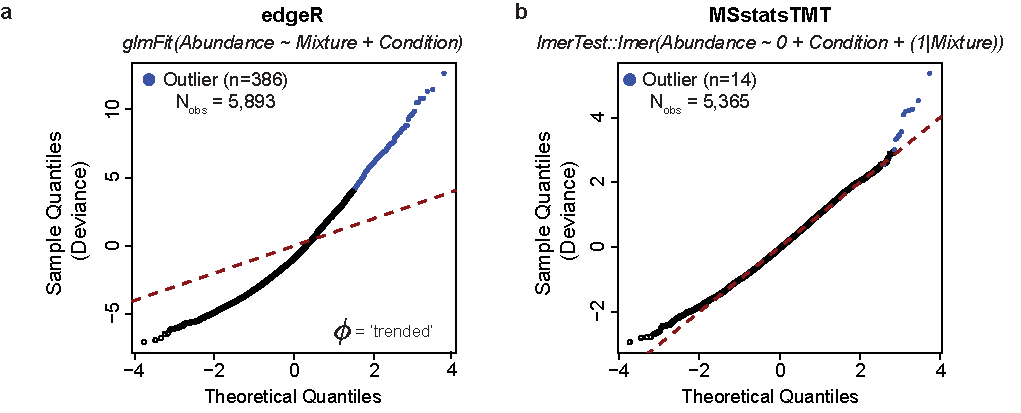
\includegraphics{fig_01}
		\caption{\textbf{Goodness-of-fit of \texttt{edgeR} (A), and 
		\texttt{MSstats} (B) statistical approaches.} The overall
		adequacy of the linear models fit to the data were assessed 
		by plotting the residual deviance for all proteins as a 
		quantile-quantile plot (McCarthy \textit{et al.}, (2012)). 
		\textbf{(A)} The normalized
		protein data were fit with a NB GLM of the form: 
		\textasciitilde{} \texttt{Mixture + Condition}.
		Where \texttt{Mixure} is a blocking factor that accounts for
		sources of variablity between experiments. Protein-wise deviance
		statistics were transformed to normality and plotted aganis
		theoretical normal quantiles using \texttt{edgeR::gof}.
		\textbf{(B)}
		The normalized protein data were fit with a linear mixed-effects 
		model (LMM) of the form: 
		\texttt{Abundance}
		\textasciitilde{}\texttt{0 + Condition + (1|Mixture)}. 
		Where \texttt{Mixture} indicates the random effect
		of \texttt{Mixture}. The residual deviance and degrees of 
		freedom were extracted from the fitted models, z-score
		normalized, and plotted as in (A). Proteins with significantly 
		poor fit are indicated as outliers in blue 
		(Holm-adjusted P-value $<$ 0.05).}
		\label{fig:gof}
	\end{center}
\end{figure}

\end{document}
